% Token Issuance
\section{Выпуск токенов (ВТ)}\label{TI}

\subsection{Обзор}\label{TI.Intro}

Пакет ВТ устанавливает требования по выбору типов токенов и их комбинаций, 
надежности токенов для соответствия тому или иному уровню гарантий 
аутентификации. 

Все рассматриваемые в настоящем стандарте токены содержат секреты 
аутентификации: статический пароль, личный или секретный ключ, другое.
%
Статический пароль способен запомнить человек, и поэтому он относится 
к фактору <<что я знаю>>. Секретные и личные ключи 
пользователь запомнить и обработать не может, они не существуют автономно,
а являются частью программного или аппаратного токена. Этот 
токен относится к фактору <<чем я владею>>.
%
Биометрические токены фактора <<кто я>> не содержат приемлемых секретов 
аутентификации. В настоящем стандарте биометрические токены могут 
использоваться только для активации аппаратных. 

\begin{figure}[bht]
\begin{center}
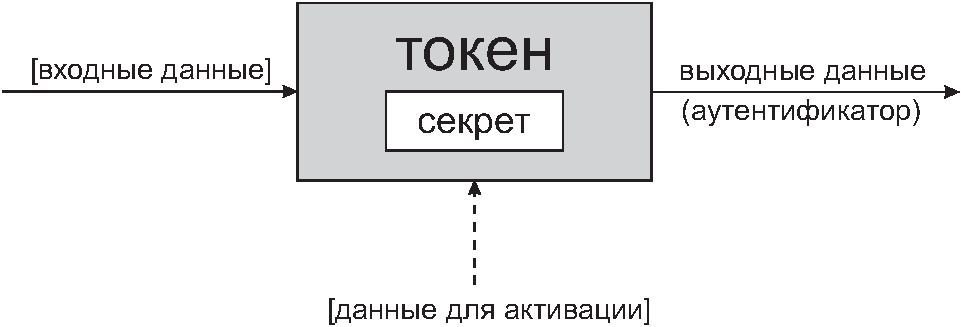
\includegraphics[width=9cm]{../figs/Token}
\end{center}
\caption{Токен аутентификации}
\label{Fig.TI.Token}
\end{figure}

Токены используются для построения аутентификаторов (см. 
\addendum{рисунок}~\ref{Fig.TI.Token}). Аутентификатор демонстрирует владение 
токеном аутентификации или его знание и, таким образом, подтверждает 
подлинность владельца.

Токены делятся на два класса: однофакторные и многофакторные.
Однофакторные токены выдают аутентификатор сразу, многофакторные~---
только после активации. Для активации нужно задействовать дополнительный 
фактор, как правило, <<что я знаю>> (PIN-код) или <<кто я>> (отпечаток пальца).

Определены следующие типы ТА.

\begin{enumerate}
\item
{\it Статический пароль}.
Секретная последовательность символов, цифр, графических элементов и пр., 
которую способен запомнить человек. 
Разделяется между пользователем и СИ.
Либо выбирается пользователем, либо генерируется СИ.
Относится к фактору <<что я знаю>>. 
Аутентификатором обычно является сам пароль.

\item
{\it Карта секретов}.
Физическое или электронное устройство, которое хранит набор секретов,
разделяемых между пользователем и СИ. Относится к фактору <<чем я владею>>. 
Аутентификатором является секрет по запрошенному СИ или выбранному 
пользователем номеру.

\item
{\it Сетевой токен}.
Устройство, связанное со СИ дополнительным соединением.
Сетевой адрес устройства зафиксирован в момент регистрации.
Относится к фактору <<чем я владею>>. 
%
Аутентификатором являются одноразовый секрет, например, пароль, который СИ
отправляет по дополнительному соединению и предлагает ввести по основному или,
наоборот, отправляет по основному соединению и предлагает ввести по
дополнительному.
%
Как правило, дополнительное соединение~--- канал GSM, сетевой адрес~--- номер
мобильного телефона пользователя.

\item
{\it Однофакторный OTP-токен}.
Аппаратное устройство или программа, которые генерируют одноразовые пароли. Для
генерации используется секретный ключ, размещенный в памяти устройства, или в
файле, сопровождающем программу. Относится к фактору <<чем я владею>>. Активация
устройства не требуется.
%
% Например, токеном может быть приложение Google Authenticator, установленное 
% на смартфоне.

\item
{\it Однофакторный аппаратный КТ}.
Аппаратный криптографический токен, который не требуется активировать.
Относится к фактору <<чем я владею>>. 

\item
{\it Программный КТ}.
Программный КТ, включающий специальный файл, в котором хранится защищенный 
секрет аутентификации. Ключ защиты строится по паролю.
%
Относится к фактору <<чем я владею>>. 
Пароль является дополнительным фактором <<что я знаю>>.

\item
{\it Многофакторный OTP-токен}.
Аппаратное устройство или программа, которые генерируют одноразовые пароли. 
Для генерации используется секретный ключ, размещенный в памяти устройства,
или в файле, сопровождающем программу. 
%
Относится к фактору <<чем я владею>>. 
%
Для активации устройства нужен дополнительный фактор <<что я знаю>> или 
<<кто я>>. 
%
Ключ хранится в файле в защищенном виде. Ключ защиты файла строится по паролю.
Пароль является дополнительным фактором <<что я знаю>>.

\item
{\it Многофакторный аппаратный КТ}.
Аппаратный криптографический токен.
Относится к фактору <<чем я владею>>. 
Для активации токена нужен дополнительный фактор <<что я знаю>> 
и/или <<кто я>>.  
\end{enumerate}

% Комбинации токенов

Пользователь может использовать несколько независимых ТА, повышая при этом 
надежность аутентификации. 

\subsection{Требования}\label{TI.Reqs}

% физический токен

\req{ВТ}{1--3}
Физический токен (карта кодов, сетевой токен, аппаратный OTP-токен или КТ)
должен сопровождаться инструкциями владельцу. Инструкции должны содержать 
сведения об обращении с токеном и о действиях в случае его пропажи или 
кражи. 

% статический пароль

\req{ВТ}{1}
Статический пароль должен содержать не менее 14 битов энтропии.
Текстовый пароль, выбираемый пользователь,
должен состоять из не менее чем 6 символов в алфавите
из 90 и более символов. Секретный PIN-код должен состоять из не менее
чем 4 цифр и должен выбираться СИ случайным образом. 
%
% 90 = numbers, alphabets and these 28 characters: 
% !"#$%&()*+,-./:;<=>?@[]^_{}~. 

% todo: псевдослучайным?

\req{ВТ}{2, 3}\label{R.TI.SP2}
Статический пароль должен содержать не менее 20 битов энтропии.
Текстовый пароль, выбираемый пользователем,
должен состоять из не менее чем 8 символов в алфавите
из 90 и более символов. Секретный PIN-код должен состоять из не менее
чем 6 цифр и должен выбираться СИ случайным образом. 

\req{ВТ}{3}
При регистрации статического пароля, выбранного пользователем, СИ должна 
проверить его отсутствие в списке паролей, которые часто используются,
ожидаемы или скомпрометированы.

% NIST SP 800-63: When processing requests to establish and change memorized 
% secrets, verifiers SHALL compare the prospective secrets against a list that 
% contains values known to be commonly-used, expected, or compromised. 

\begin{note*}
Список запрещенных паролей может включать словари распространенных паролей,
базы данных скомпрометированный паролей, тривиальные пароли из повторяющихся
или соседних символов, а также пароли, построенные по имени пользователя или 
Интернет-сервера.
\end{note*}

\req{ВТ}{1--3}
КП не должна хранить подсказки, которые помогают пользователю вспомнить забытый 
статический пароль.

% NIST SP 800-63: Memorized secret verifiers SHALL NOT permit the subscriber to 
% store a “hint” that is accessible to an unauthenticated claimant. 

\begin{note*}
При этом КП может отображать подсказки, переданные от СИ или терминала 
по защищенному соединению.
\end{note*}

\req{ВТ}{1--3}
При вводе пароля его символы (по отдельности или все вместе)
могут отображаться только на короткое время,
нужное пользователю для проверки корректности ввода.

% карта секретов

\req{ВТ}{1--3}
Карта секретов должна генерироваться СИ по секретному ключу, который содержит 
не менее 128 битов энтропии.
%
Аутентификатор карты должен содержать не менее 20 битов энтропии. 
%
Аутентификатор не должен использоваться дважды. 

% A given secret from an authenticator SHALL be used successfully only once.

% сетевой токен

\req{ВТ}{1--3}
Сетевой токен должен иметь уникальный сетевой адрес,
сообщения на который может принимать только сам токен.

\begin{note*}
\addendum{
В частности, сетевой токен не может использовать адрес электронной почты,  
поскольку сообщения на этот адрес могут принимать почтовые клиенты на разных 
устройствах. 
%
Мессенджер, который допускает установку на нескольких устройствах, также не 
может использоваться для приема сообщений.
}
\end{note*}

\req{ВТ}{1--3}
Сетевой токен должен взаимодействовать со СИ по дополнительному соединению, 
отличному от основного соединения КП~-- СИ. Дополнительное соединение 
должно быть защищено (с взаимной аутентификацией).

\begin{note*}
В настоящем стандарте не рассматривается сценарий, когда токен получает
один и тот же аутентификатор по основному и дополнительному соединениям,
и пользователь подтверждает совпадение аутентификаторов по дополнительному 
(защищенному) соединению.
\end{note*}

% todo: взаимная аутентификация в GSM?

\req{ВТ}{1--3}
Аутентификатор сетевого токена должен содержать не менее 20 битов энтропии. 
%
Аутентификатор не должен действовать более 5~\addendum{мин}. 
%
СИ должна принимать аутентификатор лишь однажды в течение периода действия.

% NIST SP800-63-3B: In all cases, the authentication SHALL be considered 
% invalid if not completed within 10 minutes.

\req{ВТ}{1--3}
\addendum{
Владелец сетевого токена должен быть проинструктирован о необходимости 
настройки токена так, чтобы в неактивном (заблокированном) состоянии токен не 
отображал аутентификаторы.}

\begin{note*}
\addendum{
Если в качестве токена выступает смартфон, то его настройка может состоять в 
подавлении отображения сообщений с аутентификаторами на экране блокировки. 
При этом уведомления о приеме сообщений можно не блокировать.}
\end{note*}

% OTP-токен

\req{ВТ}{1--3}
Для генерации одноразовых паролей в OTP-токенах должны использоваться 
механизмы HOTP или TOTP, определенные в СТБ~34.101.47. 
%
В механизмах должен использоваться секретный ключ, который содержит не менее
128 битов энтропии.
%
При использовании механизма TOTP пароль должен меняться не реже 1~раза в 
2~\addendum{мин}.
%
Пароль должен состоять из не менее чем 6 десятичных символов.

% todo: передача ключа?

\req{ВТ}{1--3}
OTP-токен должен удовлетворять требованиям СТБ~34.101.27:
программный токен~--- требованиям уровня 1 или 2,
аппаратный токен~--- требованиям уровня 3 или 4.

%OTP authenticators — particularly software-based OTP generators — SHOULD 
%discourage and SHALL NOT facilitate the cloning of the secret key onto multiple 
%devices.

% КТ

\req{ВТ}{1--3}
КТ должен удовлетворять требованиям СТБ~34.101.27:
программный токен~--- требованиям уровня 1 или 2,
аппаратный токен~--- требованиям уровня 3 или 4.
%
Секрет аутентификации должен содержать не менее 128 битов энтропии,
аутентификатор~--- не менее 64 битов.

% защита от непреднамеренных действий

\req{ВТ}{1--3}
Однофакторные аппаратные OTP-токен и КТ должны выдавать аутентификаторы 
только после физического воздействия (например, нажатия кнопки).

% активация

\req{ВТ}{1--3}
Программный КТ должен активироваться статическим текстовым  
паролем, удовлетворяющим требованию~\ref{R.TI.SP2}.
По этому паролю должен строиться ключ защиты секрета аутентификации.
Должен использоваться алгоритм PBKDF2, определенный в СТБ~34.101.45,
или схожий криптографический механизм.
%
В PBKDF2 число итераций должно быть не меньше 10000,
битовая длина синхропосылки~--- не меньше 64.

\req{ВТ}{1--3}
Многофакторные аппаратные OTP-токен \addendum{и} КТ должны активироваться 
либо статическим паролем в соответствии с требованиями~СТБ~34.101.27 (пакет ИА),
либо биометрическим токеном.
%
Биометрическая аутентификация должна удовлетворять следующим условиям:
\begin{itemize}
\item
доля ошибочных решений о соответствии биометрического образца биометрическому эталону 
не превышает 1/1000;
% 
% The biometric system SHALL operate with an FMR [ISO/IEC 2382-37] of 1 in 1000 
% or better. This FMR SHALL be achieved under conditions of a conformant attack 
% (i.e., zero-effort impostor attempt) as defined in ISO/IEC 30107-1.
%
%\item
%предусмотрена защита от атак на биометрическое предъявление (Presentation 
%Attack Detection); 
%
\item
допускается не более 5 ошибок аутентификации подряд. При достижении порога числа
неверных попыток должна выполняться либо задержка на 30~\addendum{с}, либо
переход на другой фактор аутентификации. Задержка должна увеличиваться в 2 раза
с каждой новой ошибкой аутентификации.
\end{itemize}

% комбинации

\req{ВТ}{1}
Должен использоваться токен одного из допустимых типов:
статический пароль, карта секретов, сетевой токен,
OTP-токен (однофакторный или многофакторный), 
КТ (однофакторный или многофакторный, программный или аппаратный).

\req{ВТ}{2}\label{R.TI.AAL2}
Должен использоваться многофакторный OTP-токен, программный КТ, многофакторный 
аппаратный КТ или комбинация статического пароля с одним их следующих токенов:
карта секретов, сетевой токен, однофакторный OTP-токен, 
однофакторный \addendum{аппаратный} КТ. 
%
При повторной аутентификации в рамках аутентифицированного сеанса со СИ 
достаточно дополнительно к БС использовать статический пароль.

\begin{note*}
БС выступает в роли токена фактора <<чем я владею>>.
\end{note*}

\req{ВТ}{3}
Должен использоваться многофакторный \addendum{аппаратный} КТ или одна из 
следующих комбинаций токенов:
\begin{itemize}
\item
статический пароль и однофакторный \addendum{аппаратный} КТ;
\item
многофакторный OTP-токен и однофакторный \addendum{аппаратный} КТ;
\item
\addendum{аппаратный} OTP-токен (\addendum{однофакторный или многофакторный})
и программный~КТ.
\end{itemize}

% todo: однофакторный аппаратный КТ + программный КТ?


